\chapter{Workflow}


% ---------------------------------------------------
% USED HARDWARE
\section{Used Hardware\authorA}
For video capturing a \textit{Raspberry Pi 3B+} with a \textit{Pi Camera V2} or a \textit{Pi Wide Angle Lens Camera} are used. The Raspberry Pi sends the video feed to a separate more power full PC over WiFi using a Python3 script. \newline
For processing a \textit{Lenovo Think-Station S20} or a \textit{Lenovo W550s} are used depending on the amount of processing power is required. For more intense work a server access at the Johannes Kepler University was supplied to work on their system. \newline
As the work is based around implementing it on the Audi Autonomous Driving Cup (\gls{aadc}) car a remote controlled model car was borrowed for a few weeks.


% ---------------------------------------------------
% USED SOFTWARE
\section{Used Software\authorA}
\subsection{Raspberry Pi}
The Raspberry Pi is running Raspbian Buster since it is well optimized for the mini computer and only required to be able to execute a Python script to send the raw video feed over http to the the processing device.\newline
\subsection{PC}
The Think-Station and the laptop are running Kubuntu 18.04, which is basically Ubuntu but has a GUI that's a more like Windows and is supported until May 2023. \newline
The Think-Station has a eight core Intel Xeon CPU, a GTX 1660TI and 12GB of RAM inside. \newline
The Laptop has a four core Intel i7 and 8GB of RAM built in.\newline

\textbf{\underline{ADTF}} \newline
At first Ubuntu 16.04 with Automotive Data and Time-Triggered Framework (\gls{adtf}) was used since it's the recommended environment by the \gls{aadc} car manufacturer DigitalWerk. There were many compatibility ans stability issues and it is very difficult to get into the whole system as it's not very beginner friendly. After trying to get the basics of \gls{adtf} working it was clear that switching to ROS might be better. The main problems with \gls{adtf} are, that \gls{adtf} isn't running very stable, requires certain packages to be in a non-standard folders and not having them in the regular location and it is very difficult at the when using it for the first time.

\textbf{\underline{ROS}} \newline
Running ROS Melodic on Kubuntu 18.04 was pretty straight forward. The instructions on the ROS website are very clear and can be directly copied without issues. The principle of the workspace is also easy to understand. In the source folder the modules get put in and when compiling the modules automatically generates a setup file to use them. Usage is very easy as the framework already does a lot in the background and using nodes is nearly always setting input and output with a few parameters.


% ---------------------------------------------------
% SENDING IMAGE FROM RASPBERRY PI TO PC/LAPTOP
\section{Setup\authorA}
As the PC and laptop are not the best idea to run around with, a Raspberry Pi is used instead to stream the video over WiFi to the PC/laptop which are connected to the router over LAN. This makes the camera setup very portable as the pi, camera and powerbank are packed together and don't have much weight. The PC can sit somewhere where and just processing the received video signal.
\begin{figure}[h]
	\centering
	\includegraphics[width=0.8\textwidth]{./media/images/PiSetup.png}
  	\caption{Stream setup with Raspberry Pi, camera and powerbank}
  	\label{picamssetup}
\end{figure}

\section{Streaming video from Pi to PC\authorA}

\textbf{\underline{Enabling Camera}}\newline
To use a camera on a Raspberry Pi the interface needs to be enabled first. This can be done in the built-in tool called \textit{raspi-config}. In this tool under the subsection called \textit{Interfacing Options} there is a option with the name \textit{Camera}. When this is done the camera can be used after a restart.

\textbf{\underline{Python Script}}\newline
In the code snipped \ref{code:videostreamMain} at first a \textit{piCamera} instance with the name \textit{cam} is created. As parameters the resolution gets set to \textit{1280x720} pixels and the frame rate is set to \textit{30} frames per second (\gls{fps}). If needed the image can be rotated, e.g the camera is mounted upside down. When starting the camera a output and format are expected. For the output a separate class is used which sets how and when a new frame can be published and for the format the \textit{mjpg} video codec is chosen, as a pack for getting MPEG-streams already exists in \gls{ros} and it's not power hungry when running it on the Raspberry Pi. \newline
After the camera \enquote{recording} has started successfully the server is started to make the stream accessible to other devices. The server runs until the user closes the script using \textit{CTRL + C}. After closing the server the \textit{finally} block gets called, where the camera \enquote{recording} is stopped so that other programs can use the camera again.
\lstinputlisting[language=Python, firstline=77, lastline=91,caption={Main Function of Camera Feed},label={code:videostreamMain}]{./media/code_snippets/HTTPCamStream.py}

The streamingHandler that is shown in snipped \ref{code:videoStreamHandler} handles the actions that are taken when client connects to the Raspberry Pi. At the beginning it checks if the client is requesting the \textit{/stream.mjpg} file. If the client is not requesting that specific file a \textit{404 Not Found} Error is returned. But if the correct file is requested at first a \textit{200 OK} code. In addition to the status code headers are send, which tell the client to not use cache. After sending the HTTP OK to the client a permanent loop is started which always waits until a new image from the camera is ready and then sends it to the client as an JPEG image. The loop ensures that the always client receives the latest image and so creates a video. Should the client drop the connection an exception is raised which causes the loop to stop and end the handler for that specific client until the client connects again.
\lstinputlisting[language=Python, firstline=42, lastline=74, caption={Streaming Handler of CamStream},label={code:videoStreamHandler}]{./media/code_snippets/HTTPCamStream.py}

The behavior when a new image from the pi camera is ready to send is defined in the snipped \ref{code:videoStreamingOutput}. At the beginning it initializes itself with basically no image. \textit{piCamera} class constantly writes into this, as it's defined as the output. When a new image is ready the \textit{picamera} class sends \enquote{\textbackslash xff\textbackslash xd8} as binary to the output class to notify it. The output class then cuts the buffer so it only contains the current image and sets it in the \textit{frame} variable. To let everybody else know that a new image is ready it sends out a notification.
\lstinputlisting[language=Python, firstline=26, lastline=40, caption={Streaming Output of CamStream},label={code:videoStreamingOutput}]{./media/code_snippets/HTTPCamStream.py}


% ---------------------------------------------------
% RECEIVING IMAGE ON PC/LAPTOP
\section{Receiving images on PC and Laptop\authorA}
For receiving the images on the PC or Laptop an existing \gls{ros}-node is used. Video-Stream-OpenCV is designed to publish videos in the \gls{ros} network which are received from different sources, e.g. USB-cameras, video-files, network cameras and video-streams \cite{videostreamopencv}.

\subsection{MJPG-Stream receiver}
To automate the startup procedure of the node a roslaunch file is used to start the node is written for and automatically sets the required parameters.\newline
The launchfile shown in \ref{code:mjpgstreamreceiverlaunch} published the received image stream on a topic called \textit{camera}. The video stream provider are the Raspberry Pi's IP-address, port and \textit{/stream.mjpg} directory. 30 \gls{fps} are used since they provide a good balance between amount of traffic and amount of detail in the movement.
\lstinputlisting[language=XML, firstline=3, lastline=14, caption={MJPG-Stream receiver Launch file},label={code:mjpgstreamreceiverlaunch}]{./media/code_snippets/mjpg-stream.launch}


% ---------------------------------------------------
% Cameras
\section{Cameras\authorA}
Nearly every camera has some kind of distortion where the proportions of the image are different to the real world. This is especially noticeable on wide angle lenses which can capture a bigger part of the environment while sitting in the same spot. This can be seen in figure \ref{cameracomparison} that the normal camera only captures a small portion compared to the wide angle lens camera but the wide angle lens creates distortions when getting to the edges.
\begin{figure}[h]
	\centering
	\includegraphics[width=0.8\textwidth]{./media/images/CameraComparison.png}
  	\caption{\textbf{Left Image:} normal Raspberry Pi Camera. \textbf{Right Image:} wide angle lens camera}
  	\label{cameracomparison}
\end{figure}

\subsection{Calibration}
To get rid of the distortions on a wide angle lens camera calibration is needed, which is a mask that gets applied on the image to remove these distortions and rectify it.
For calibration the \textit{camera calibration}-node is used.  Calibration is done by moving and rotating a checkerboard is used since it has good contrast between the tiles and the size of a tile is known and always the same. The node recognizes the checkerboard and calculates the distortion-factors from a series of pictures that have been taken.\newline
The command for starting the node is the following, where amount of tiles, size of tiles in millimeter and camera are set:
\begin{lstlisting}[language=BASH,caption={Start Calibration Node}]
rosrun camera_calibration cameracalibrator.py --size 8x6 --square 0.026 --no-service-check image:=/camera/image_raw camera:=/camera
\end{lstlisting}
b
This command opens a window which shows the live image feed from the camera and highlights edges on the checkerboard which is shown in figure \ref{cameracalibration}. These highlighted edges are points which are used to calculate the distortion parameters using an algorithm that was developed by OpenCV \cite{cameracalibrationopencv}.
\begin{figure}[h]
	\centering
	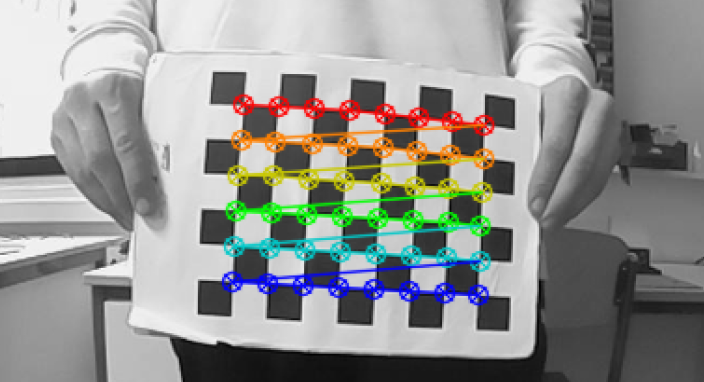
\includegraphics[width=0.8\textwidth]{./media/images/CameraCalibration.png}
  	\caption{Camera calibration}
  	\label{cameracalibration}
\end{figure} \newline

When the node has enough reference images the computing of the parameters can start. The duration of the calculations depends on the CPU and how many images have been taken. But most likely it will take around 5 Minutes until the computing is finished. The output data contains two formats of the same data which will look something like shown in figure \ref{code:calibrationyaml}. The output files are normally compatible with all applications without any issues.
\lstinputlisting[language=XML, firstline=1, lastline=14, caption={Calibration file},label={code:calibrationyaml}]{./media/code_snippets/calibration.yaml}


% ---------------------------------------------------
% Running ORB-SLAM2
\section{Running ORB-SLAM2}\label{ref:runningorbslam}
Integrating ORB-SLAM2 \ref{ref:orbslam} is pretty straight forward since there is already \gls{ros} version of it which is very well maintained by \textbf{appliedAI-Initiative} on GitHub \cite{orbslam2rosgithub}. It just needs to be cloned into the \textit{src} folder of the \gls{ros}-workspace and complied using the \textit{catkin build} command. \newline

\subsection{Calibration file}
When building the packs is finished the generated setup-file has to be sourced. The file is located under \textit{workspace/devel/setup.sh} and can be sources using the \textit{source setup.sh} command. After sourcing the setup all new types of commands that are added by the nodes are available.\newline
Before using the ORB-SLAM the calibration file needs to be created in \textit{src/orb\textunderscore slam2/config/config.yaml}. For a baseline the config from another mono-camera can be copied. The calibration part looks like shown in \ref{code:orbslamconfig} and thus the config that the calibration tool generated needs to be converted manually. In the camera\textunderscore matrix the values are the following: \textsc{[\textbf{camera.fx}, 0, \textbf{camera.cx}, 0, \textbf{camera.fy}, \textbf{camera.cy}, 0, 0, 1]}. The distortion\textunderscore coefficients need to be mapped like this \textsc{[\textbf{camera.k1}, \textbf{camera.k2}, \textbf{camera.p1}, \textbf{p2}, 0]}. Additionally the width, height and \gls{fps} of the incoming video have to be set.\newline
\lstinputlisting[language=XML, firstline=3, lastline=17, caption={ORB-SLAM2 config calibration}, label={code:orbslamconfig}]{./media/code_snippets/config.yaml}

\subsection{Launching ORB-SLAM2}
To load the new config file a new launch file is the best way to tell the \gls{slam} to use this config instead of the default parameters. The launch files for ORB-SLAM2 sit in \textit{src/orb\textunderscore slam2/ros/launch} where an existing one can be duplicated. The new launch-file should look like the snipped \ref{code:orbslam2launch} except in line \textbf{13} the wrong config is specified. Additionally in the config other settings can be set. For example if the node should publish a pointcloud or position, only do tracking. It is also possible to load an existing map which has been created before and might be used to add additional information or do tracking only on it. When everything is configured it is now possible to launch the ORB-SLAM2 using \textit{roslaunch orb\textunderscore slam2\textunderscore ros orbslam.launch}. \newline
\lstinputlisting[language=XML,  caption={ORB-SLAM2 launch file}, label={code:orbslam2launch}]{./media/code_snippets/orbslam.launch}

When starting RQt \ref{rqt} and opening the \textsc{Node Graph} it should show, like seen in figure\ref{img:nodegraphstreamorbslam} that the camera-node is sending \textit{image\textunderscore raw} to the \textit{orb\textunderscore slam2\textunderscore mono}-node. If that is not the case it is most likely due to some spelling error or a \textit{remap} line in the launch-file of the ORB-SLAM2.\newline
\begin{figure}[h]
	\centering
	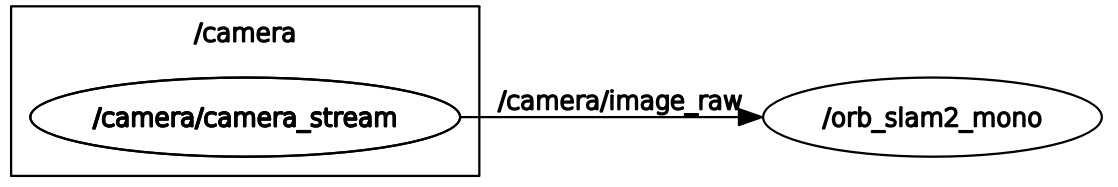
\includegraphics[width=0.8\textwidth]{./media/images/nodegraphstreamorbslam.png}
  	\caption{Node Graph with Stream and ORB-SLAM}
  	\label{img:nodegraphstreamorbslam}
\end{figure}



% ---------------------------------------------------
% Running LSD-SLAM
\section{Running LSD-SLAM}
Running the LSD-SLAM is not as straight forward as it is on the ORB-SLAM \ref{ref:runningorbslam}. The implementation of the LSD-SLAM is made to use it with \gls{ros} out of the box but the original version by the Computer Vision Group at the Technical University of Munich was not updated in the past 5 years and such had some problems when running it on a newer version of \gls{ros} and Ubuntu. Therefor an more up-to-date version by Kevin George \cite{kevingeorgelsdslam} was used where he added support for newer versions of libraries and fixed some bugs. Even though the fork by Kevin George was updated 2 Years ago there were still some bugs and other problems. So a fork was created with the fixes to address the problems that where in Kevin George's Repository. The fork includes bug fixes to run LSD-SLAM on \gls{ros}-Melodic and Ubuntu 18.04 pretty much out of the box.\newline

The fork\cite{alexandervoglspergerlsdslam} contains implementation to use \textsc{Eigen v3.2.5} that doesn't need to be installed, a special version of General Graph Optimization (\gls{g2o}) and a \textsc{CSPARSE}-directory path fix.\newline

\subsection{Installing LSD-SLAM}
To run the LSD-SLAM a few packages are required. They can be installed using\newline
\begin{lstlisting}[language=bash]
    apt install ros-melodic-cv-bridge liblapack-dev libblas-dev freeglut3-dev libqglviewer-dev-qt4 libsuitesparse-dev libx11-dev
\end{lstlisting}

and then creating a link for \textit{libQGLViewer} to the file the LSD-SLAM is looking for. To create the softlink this command is used wich basically creates a link just without the \textsc{-qt4} at the end.\newline
\begin{lstlisting}[language=bash]
    sudo ln -s /usr/lib/x86\textunderscore 64-linux-gnu/libQGLViewer-qt4.so /usr/lib/x86\textunderscore 64-linux-gnu/libQGLViewer.so
\end{lstlisting}

As the LSD-SLAM requires a special version of the \gls{g2o} framework all other versions that have been installed on \gls{ros} need to be removed completely. For this first the \textit{ros-melodic-g2o} package needs to be purged and the leftovers need to be deleted to not conflict with the special version that is going to be installed later using.\newline
\begin{lstlisting}[language=bash]
    rm -r /usr/local/lib/libg2o* /usr/local/include/g2o /usr/local/lib/g2o /usr/local/bin/g2o*
\end{lstlisting}

To install the correct version of \gls{g2o} it needs to be cloned from \url{https://github.com/felixendres/g2o.git} which creates a g2o folder in which a \textit{build}-folder has to be created. In the \textit{build} folder two commands have to be executed in order to install the framework.\newline
\begin{lstlisting}[language=bash]
    cmake ..
    sudo make install
\end{lstlisting}

When done it is also necessary to download a specific version of the \textsc{Eigen}-library which has to be in a location where it is not likely to be moved as the full path is required. The Path should look a bit like this \textit{/home/alex/Projects/LSD-SLAM/eigen-eigen-bdd17ee3b1b3/}. This path needs to be set in the \textit{CMakeList.txt} in the \textit{lsd\textunderscore slam\textunderscore core} folder which was contained in the LSD-SLAM repository. In the file at line \textbf{106} there should be a placeholder like shown in \ref{code:eigenpathdir}, which has to be replaced with the path of \textsc{Eigen}.\newline
\lstinputlisting[language=XML, firstline=106, lastline=106, caption={CMakeList Eigen Directory}, label={code:eigenpathdir}]{./media/code_snippets/LSD-SLAM-Core-CMakeList.txt}

When these steps are done there is only one last command to be executed in the root directory of the workspace. To compile the LSD-SLAM in the src folder the command is \newline
\begin{lstlisting}[language=bash]
    catkin_make
\end{lstlisting}
which may take some time. 